\documentclass[journal, onecolumn]{IEEEtran}

\renewcommand\IEEEkeywordsname{Keywords}

\usepackage{graphicx}
\graphicspath{ {images/} }
\usepackage{tabularx}
\usepackage{pdfpages}
\usepackage{amsmath}

\pagenumbering{arabic}
\bibliographystyle{IEEEtran}

\begin{document}
	\markboth{COMPSYS701 - Advanced Digital Systems Design}{}
	
\begin{titlepage}
	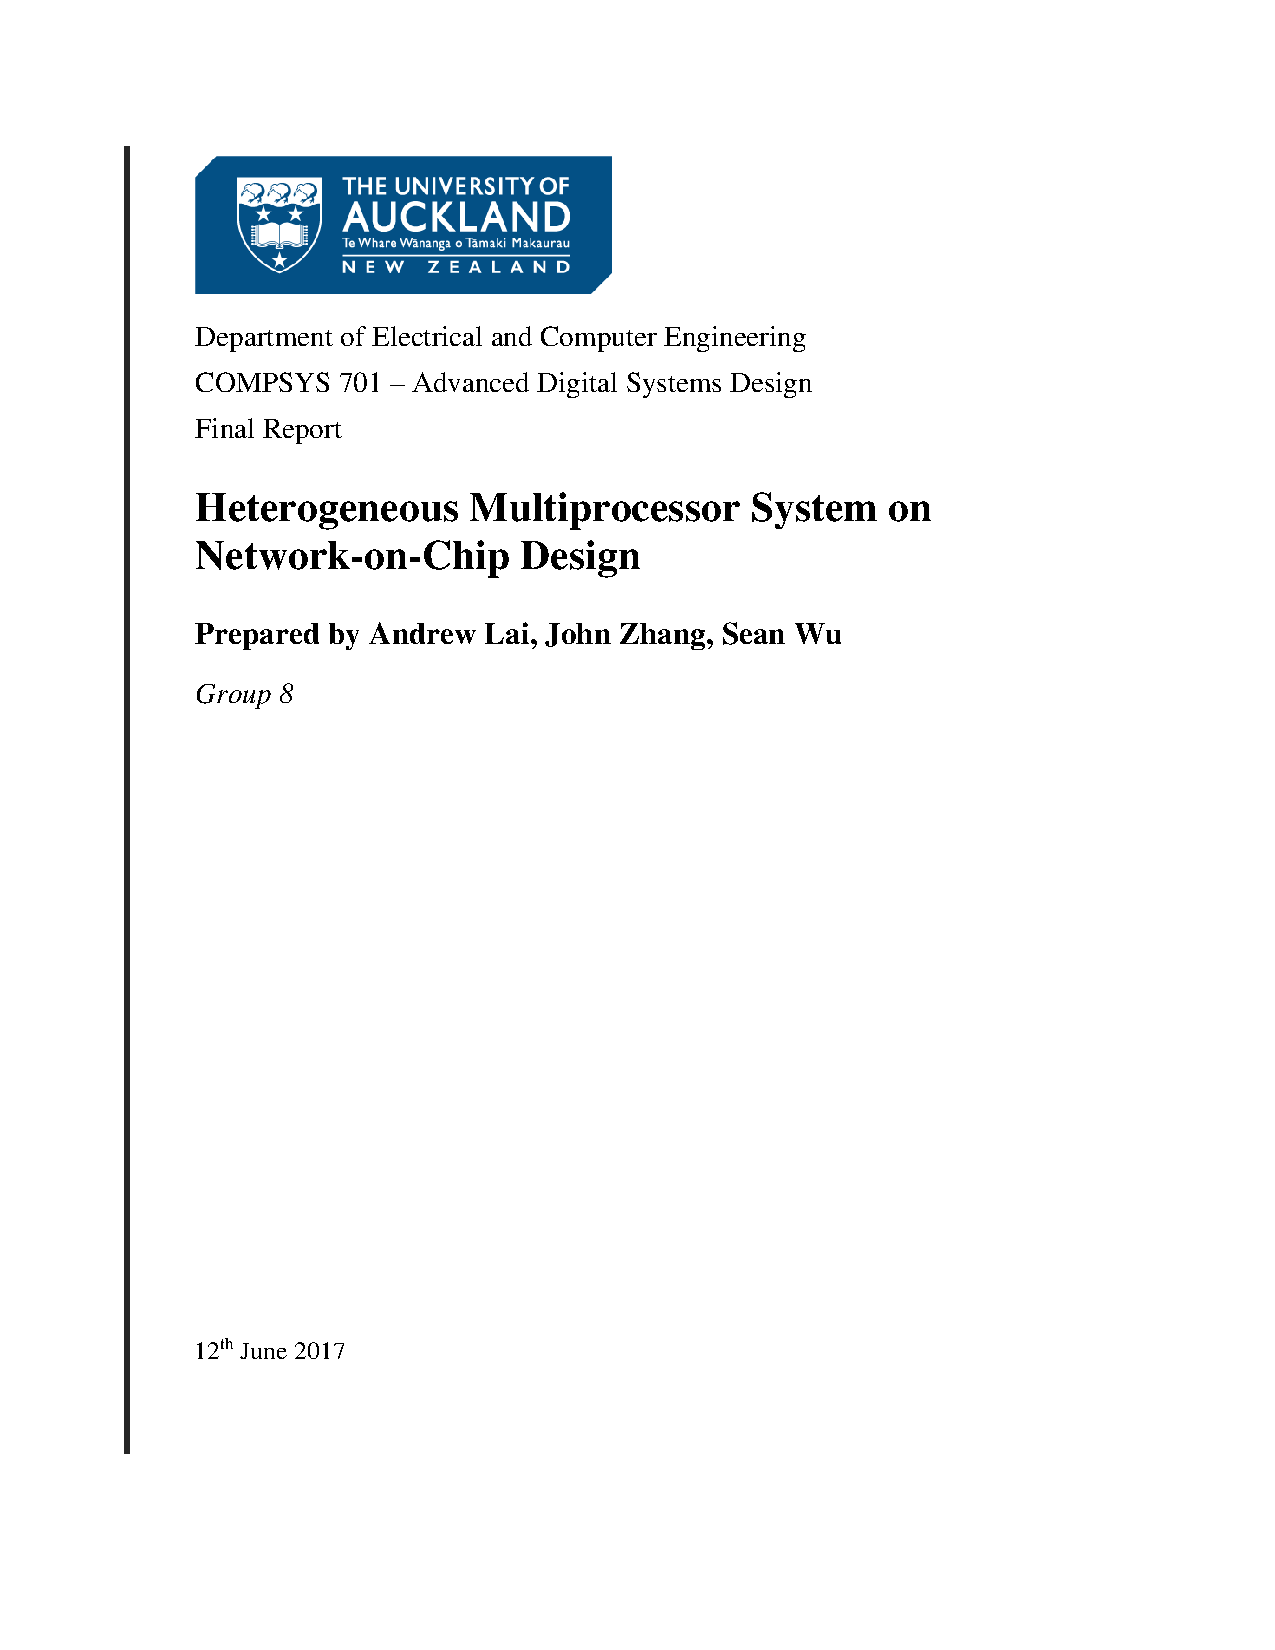
\includepdf[pages={1}]{title_page.pdf}
\end{titlepage}

	\setcounter{page}{2}
	
	\title{Heterogeneous Multiprocessor System on Network-on-Chip Design}
	\author{Andrew Lai \texttt{(klai054)}, John Zhang \texttt{(szha215)}, Sean Wu \texttt{(swu145)}, group 8 - AJS \\Department of Electrical and Computer Engineering, University of Auckland, New Zealand}
	
	\maketitle
	
	\begin{abstract}
		Processors architecture size and maximum frequencies are hitting their limits. To further improve performance, multi-core systems are required.
	\end{abstract}
	
	\begin{IEEEkeywords}
		Processor design; Network-on-chip 
	\end{IEEEkeywords}
	
	
	\section{Introduction}
	
%	\begin{figure}[h!]
%		\centering
%		\includegraphics[trim={0cm, 0cm, 0cm, 0cm}, clip, width = 3.4in]{pedal_detection_fsm}
%		\caption{Pedal Detection FSM.}
%		\label{tumor_L8}
%	\end{figure}
	
	
	\section{Network-on-Chip Structure}
	
		\subsection{Basic Architecture}
		
		\subsection{Configuration}
	
	\section{Reactive Coprocessor (AJS)}
		
		\subsection{Control Unit}
		
		\subsection{Datapath}
		
		\subsection{Data Format}
		
		\subsection{Simulation}
	
	
	\section{Application Specific Processor}

		\subsection{Control Unit}

		\subsection{Datapath}

		\subsection{Operations}
		
		\subsection{Data Format}

	\section{ASP Network Interface}

		\subsection{Datapath}
		
		\subsection{Interaction with TDMA-MIN}
		
		\subsection{Timing}
				
		\subsection{Simulation}
		
		\subsection{Sythesis}
		
		\subsection{FPGA Testing}

		\subsection{Performance Analysis}
		
		

	\section{JOP Network Interface}



	\section{Java Programmes}

		\subsection{ASP APIs}

	\section{SystemJ Integration}



	\section{Performance Analysis}


	
	\section{Conclusion}



	\section{Acknowledgements}
	
	
	
	\section{References}
	
	
	
	\section*{Appendix}
	
	
	
\end{document}

